\documentclass[10.5pt,a4paper]{article}
\usepackage[margin=2.2cm]{geometry}
\usepackage{amsmath,amssymb,mathtools}
\usepackage{booktabs,tabularx,array}
\usepackage{graphicx}
\usepackage{xcolor}
\usepackage{enumitem}
\usepackage[hidelinks]{hyperref}
\usepackage{caption}
\usepackage{pdflscape}
\usepackage{placeins}
\captionsetup{font=small,labelfont=bf}
\setlist{itemsep=2pt,topsep=3pt}
% \input is not expandable inside tabular; the TeX primitive is
\makeatletter\let\inputrows\@@input\makeatother
\newcolumntype{Y}{>{\raggedright\arraybackslash}X}
\definecolor{note}{HTML}{F2F1EC}
\definecolor{todo}{HTML}{FBE9E0}
\newcommand{\callout}[1]{\par\smallskip\noindent\colorbox{note}{\parbox{\dimexpr\linewidth-2\fboxsep}{\small #1}}\par\smallskip}
\newcommand{\pending}[1]{\par\smallskip\noindent\colorbox{todo}{\parbox{\dimexpr\linewidth-2\fboxsep}{\small\textbf{Pending.} #1}}\par\smallskip}

\title{\textbf{CT-KAE: the two candidate models}\\[2pt]
\large Reference and back001, mixture readout, ablations, data assimilation and post-processing}
\author{Prepared for R.~Grozavescu}
\date{28 October 2026}

\begin{document}
\maketitle

\section*{The short version}

\textbf{Two candidates.} Both are the same continuous-time Koopman autoencoder (CT-KAE) with
exactly linear latent dynamics, read out with a train-calibrated \emph{mixture} readout:
\begin{itemize}
\item the \textbf{reference}: trained on reconstruction, 8-lead prediction, latent consistency
  and amplitude matching;
\item \textbf{back001}: the same, plus the original KAE's \emph{backward latent consistency} at
  weight 0.01.
\end{itemize}

\begin{center}\small
\begin{tabular}{lcccc}
\toprule
 (MSE $\times10^{-3}$, all frames; DA: mean over 37 df9 points; lower is better)
 & Tra\_ext & Tra\_int & Tra\_long & DA df9\\
\midrule
ACDM (official)                      & 2.14 & 2.92 & 22.63 & 0.258\\
U-Net$_{ut}$ (official)               & 1.60 & \textbf{1.48} & 22.18 & 0.270\\
U-Net$_{tn}$ (official)               & \textbf{1.37} & 1.77 & 22.38 & --\\
Original KAE (final checkpoint)       & 2.05 & 11.05 & 18.47 & 0.103\\
CT-KAE reference + mixture (mean of 3 seeds)  & 1.77 & 3.16 & 13.03 & 0.095\\
back001 + mixture (mean of 3 seeds)           & 1.88 & 2.89 & 13.45 & \textbf{0.088}\\
\midrule
\multicolumn{5}{l}{\emph{With post-processing (\S\ref{sec:pp}; forecasts only, train-calibrated)}}\\
reference, 3-seed average + mixture + shrink  & 1.58 & 2.92 & \textbf{11.97} & --\\
back001, 3-seed average + mixture + shrink    & 1.69 & 2.66 & 12.04 & --\\
\bottomrule
\end{tabular}
\end{center}

\begin{itemize}
\item \textbf{Long rollouts:} both candidates beat every baseline by about 40\%.
\item \textbf{Data assimilation:} both are about 3$\times$ more accurate than ACDM and U-Net, and
  back001 is the best model tested, better than the reference on 36 of 37 df9 points.
\item \textbf{Short-horizon forecasts (ext, int):} the U-Nets remain best; back001 + mixture is
  the best CT-KAE on int and just ahead of ACDM there.
\item \textbf{back001 against the reference} (paired, 3 seeds): DA $-0.0076\pm0.0040$, int
  $-0.27\pm0.10$, ext $+0.11\pm0.20$ (tie), long $+0.42\pm0.12$. It improves the two metrics
  ranked first (DA, then MSE on int) and costs 3\% on long; it fails the pre-registered
  rule (lower DA \emph{and} no worse on ext/int/long) on long only.
\item \textbf{LSiM} gets worse with the mixture readout for both models (it softens long-lead
  fields); on LSiM the baselines win throughout.
\item \textbf{Post-processing} (\S\ref{sec:pp}): averaging the three seeds is the largest gain
  (ext $-10\%$, int $-8\%$, long $-3$ to $-4\%$), and shrinking the long-lead forecast towards a
  Mach-matched training climatology adds a further 6--9\% on long. Together they take the
  reference to 1.58 / 2.92 / 11.97 and back001 to 1.69 / 2.66 / 12.04. Both cost LSiM.
\end{itemize}

\callout{\textbf{Recommendation.} Keep both. Use \textbf{back001 + mixture} where data
assimilation and short/medium-range accuracy matter (it is the DA model of the paper), and the
reference + mixture as the best long-rollout model. For the best forecasting numbers, report each
as a \textbf{3-seed average} with the mixture readout and \textbf{climatology shrinkage}: every
member stays an exact linear model, everything is calibrated on training data, and the cost is
3$\times$ inference. Report the single-model numbers alongside, and LSiM for both, since the
post-processing lowers MSE by smoothing. With shrinkage, back001's long-rollout deficit against
the reference drops from 0.42 to 0.09 (single-seed means).}

\tableofcontents

%======================================================================
\section{The model}\label{sec:model}

\subsection{Architecture}
\begin{equation*}
z_0 = E(x_{t-1}, x_t;\,\mathrm{Ma}),\qquad
z(\tau) = e^{\tau A(\mathrm{Ma})} z_0,\qquad
\hat x(t+\tau) = D(z(\tau);\,\mathrm{Ma}).
\end{equation*}
\begin{itemize}
\item \textbf{Encoder} (12.1\,M parameters). Input: 2 frames $\times$ 4 fields, the obstacle mask
  and two coordinate channels (11 channels, $64\times128$). Three CNN stages (widths 64/128/256),
  two residual blocks each (GroupNorm, SiLU, $3\times3$ convolutions), stride-2 downsampling to
  $8\times16$, flatten, one linear layer to $z\in\mathbb R^{256}$. Every residual block is
  FiLM-modulated by a 64-dimensional embedding of $(\mathrm{Ma}-0.7)/0.1$, zero-initialised.
\item \textbf{Latent dynamics} (21\,k parameters). 128 independent damped oscillators,
  $A=\mathrm{blockdiag}_j\begin{psmallmatrix}-\gamma_j & -\omega_j\\ \omega_j & -\gamma_j\end{psmallmatrix}$,
  $\gamma_j(\mathrm{Ma})=\mathrm{softplus}(\cdot)\ge0$ (no growing modes), $\omega_j(\mathrm{Ma})$
  free; both are a base value plus a zero-initialised Mach correction. No fixed-point offset.
\item \textbf{Decoder} (12.6\,M parameters). Mirror of the encoder with FiLM; the only nonlinearity
  between $z$ and the pixels.
\end{itemize}

\subsection{The latent dynamics are exactly linear}
$e^{\tau A}$ is evaluated in closed form, $e^{-\gamma_j\tau}$ times a rotation by $\omega_j\tau$ per
block; this \emph{is} the matrix exponential. Checked on the trained back001 (seed 0, Ma 0.66)
against \texttt{torch.linalg.matrix\_exp} in float64:

\begin{center}\small
\begin{tabular}{lcccccc}
\toprule
$\tau$ (time units) & 0.1 & 1.0 & 5.8 & 23.8 & $-5.0$ & $-23.8$\\
\midrule
rel.\ difference, float64 & 2e-16 & 1e-15 & 5e-15 & 2e-14 & 6e-15 & 3e-14\\
rel.\ error, float32 (as used) & 5e-8 & 6e-8 & 4e-7 & 1e-6 & 3e-7 & 4e-6\\
\bottomrule
\end{tabular}
\end{center}
Semigroup $e^{1.0A}e^{5.8A}=e^{6.8A}$: $6\times10^{-16}$; linearity: $3\times10^{-17}$; largest
real part of the spectrum: $-4.5\times10^{-5}$. The block form loses no generality beyond
growing modes, Jordan blocks and paired equal real eigenvalues (any diagonalisable real $A$ is
similar to it, and the similarity is absorbed by the encoder and decoder).

\subsection{Training}
\begin{center}\small
\begin{tabularx}{\linewidth}{lcY}
\toprule
Term & Weight & What it enforces\\
\midrule
rec & 1 & $D(E(\text{window}))$ reproduces the window's last frame\\
pred & 1 & $D(z(\tau_k))$ matches the true frame at each of the 8 leads (0.1 apart)\\
lat & 0.1 & $z(\tau_k)$ matches the stop-gradient encoding of the true window at $\tau_k$
  (normalised by $E|z|^2$)\\
amp & 0.1 & oscillator amplitudes $|(a_j,b_j)|$ match the encoded ones\\
\textbf{back} (back001 only) & \textbf{0.01} & encode the last window of the clip, propagate
  \emph{backward} to every earlier lead and to $t_0$, match the stop-gradient encodings\\
\bottomrule
\end{tabularx}
\end{center}
Channel-weighted squared error; 20\,k steps, batch 16, AdamW ($3\times10^{-4}$, weight decay
$10^{-4}$, 500-step warm-up, cosine to 5\%), gradient clip 1, bf16. Data: the 33 ACDM training
simulations (train.nc plus simulation 40), all frames, random offsets, no validation split,
final checkpoint (the ACDM protocol). 24.7\,M parameters; about 3 GPU hours per seed.

\subsection{Mixture readout (inference only)}
The forecast averages 5 decodes of the same linear flow run with all frequencies scaled by
$s_q=1+\sigma\xi_q$ (Gauss--Hermite nodes and weights):
$\hat x(\tau)=\sum_q w_q\,D\!\left(e^{\tau A_{s_q}}z_0\right)$. Every decoded latent is a real
trajectory of the model; the averaging is in pixel space. $\sigma$ is chosen per checkpoint
on training rollouts only (\S\ref{sec:mix}). Training is unchanged, the same checkpoint
gives both readouts ($\sigma=0$ is the single decode), and DA does not use the readout.

\subsection{Data assimilation}
Strong-constraint latent 4D-Var: the control is $z_0$ only, the misfit
$\|H D(e^{\tau_j A}z_0)-y_j\|^2$ over observations 0.9--5 time units after $t_0$ (df9) or from
one frame after $t_0$ (df1) is minimised with Adam from $z=0$ for 500 iterations, learning
rate tuned per model on gt\_extrap; the analysis $D(z_0)$ at the unobserved $t_0$ is scored
on gt\_interp (8 problems per point).

%======================================================================
\section{Comparison with the baselines}\label{sec:main}

\begin{table}[h]
\centering\scriptsize
\caption{Test set, same cases and scorers for every model. MSE $\times10^{-3}$ on all frames
(ACDM-paper convention); LSiM $\times10^{-1}$; DA: mean analysis error over the 37 points of the
six df9 sweeps (noise, sparsity, window length, number of observation times, misspecified
noise, joint sparsity). CT-KAE rows: mean $\pm$ s.d.\ over 3 seeds. Lower is better.
$^\ast$Selected on forecast loss on gt\_interp, the trajectories DA is tested on; its DA is
therefore optimistic. Original KAE forecasts: final checkpoint re-run through the verified
pipeline (the stored prediction files are not reproducible); its LSiM was not computed.}
\label{tab:main}
\resizebox{\linewidth}{!}{%
\begin{tabular}{lccccccc}
\toprule
 & \multicolumn{3}{c}{MSE} & \multicolumn{3}{c}{LSiM} & DA\\
\cmidrule(lr){2-4}\cmidrule(lr){5-7}
Model & Tra\_ext & Tra\_int & Tra\_long & Tra\_ext & Tra\_int & Tra\_long & df9 (37 pts)\\
\midrule
\inputrows tab_main.tex
\bottomrule
\end{tabular}}
\end{table}

\begin{figure}[h]
\centering
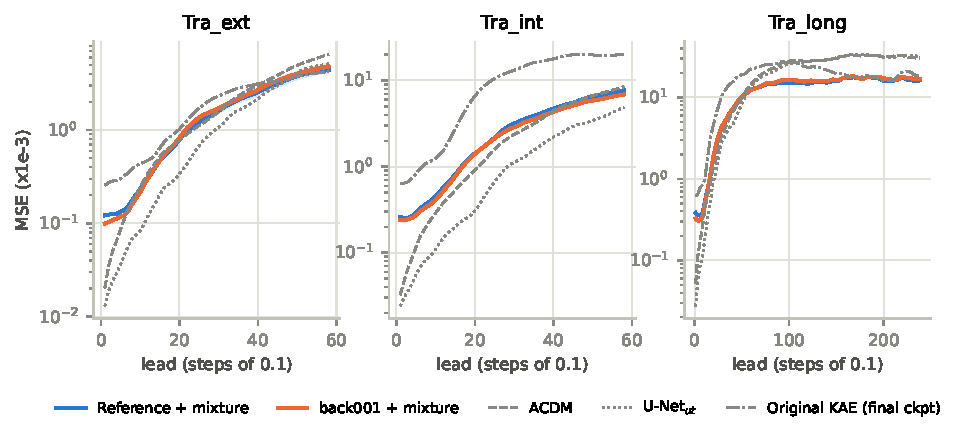
\includegraphics[width=\linewidth]{fig_cand_lead.pdf}
\caption{MSE per lead (log scale), CT-KAE: mean over 3 seeds with $\pm$SE band, both with the
mixture readout. The CT-KAEs start above the U-Nets at short leads (the encoding floor,
\S\ref{sec:findings}) and stay far below every baseline beyond about 60 leads.}
\label{fig:lead}
\end{figure}

%======================================================================
\section{back001 against the reference}\label{sec:back001}

\subsection{Forecasting, lead by lead}
\begin{figure}[h]
\centering
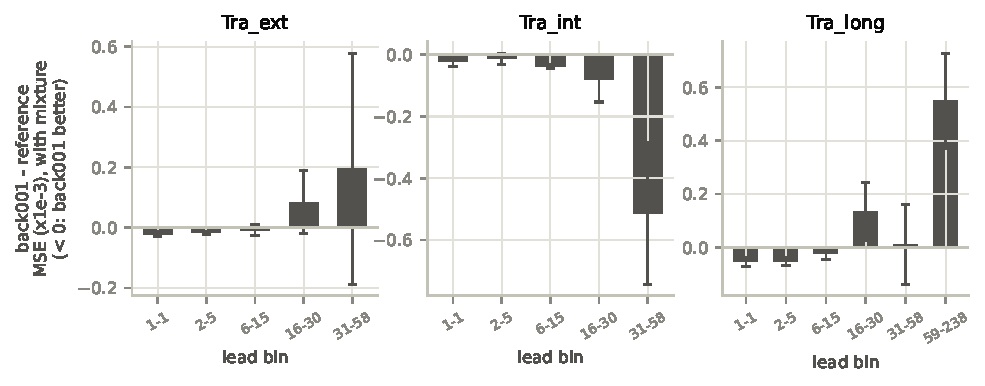
\includegraphics[width=\linewidth]{fig_cand_delta.pdf}
\caption{Paired difference back001 $-$ reference by lead bin, mixture readout, mean $\pm$ SE
over 3 seeds; negative means back001 is better.}
\label{fig:delta}
\end{figure}

\begin{itemize}
\item \textbf{Leads 1--15: better everywhere.} Lead-1 MSE 0.122$\to$0.100 (ext, $-18\%$),
  0.259$\to$0.238 (int, $-8\%$), 0.382$\to$0.327 (long, $-15\%$), negative in nearly every seed.
  Lead 1 is almost pure encoding and decoding, so the backward term mainly yields a more accurate
  encoder.
\item \textbf{int, leads 31--58: better}, $-0.51\pm0.23$ (anomaly correlation 0.804$\to$0.823).
\item \textbf{ext, leads 16--58: worse on average} (+0.08, +0.20) but one seed reverses sign:
  seed noise rather than a consistent loss.
\item \textbf{long, leads 59--238: the only real loss}, $+0.55\pm0.18$ with the mixture (all
  three seeds), although without the mixture back001 is better there ($-1.29\pm1.19$,
  19.69$\to$18.40). back001 gains less from the mixture ($-2.05$ against $-3.9$).
\end{itemize}

\textbf{Why long gets worse.} back001 learns more damping (median $\gamma$ 0.058 against 0.045,
e-folding time 17 against 22 time units; $|\omega|$ range almost unchanged). Part of its
long-lead hedging is therefore latent damping, the weaker of the two hedges (pixel-space
averaging of phases beats latent shrinkage, \S\ref{sec:findings}), and the mixture has less phase
error left to average. The same pattern appears on 238-lead \emph{training} rollouts (single
decode 11.07 vs 11.05, best mixture 9.93 vs 10.11; Figure~\ref{fig:sigma}), so it is a property
of what back001 learned, not of the readout calibration: re-calibrating $\sigma$ on 238-lead
training rollouts returns the same $\sigma$ (0.04 / 0.04 / 0.05) for all six checkpoints.

\subsection{Data assimilation}
\begin{figure}[h]
\centering
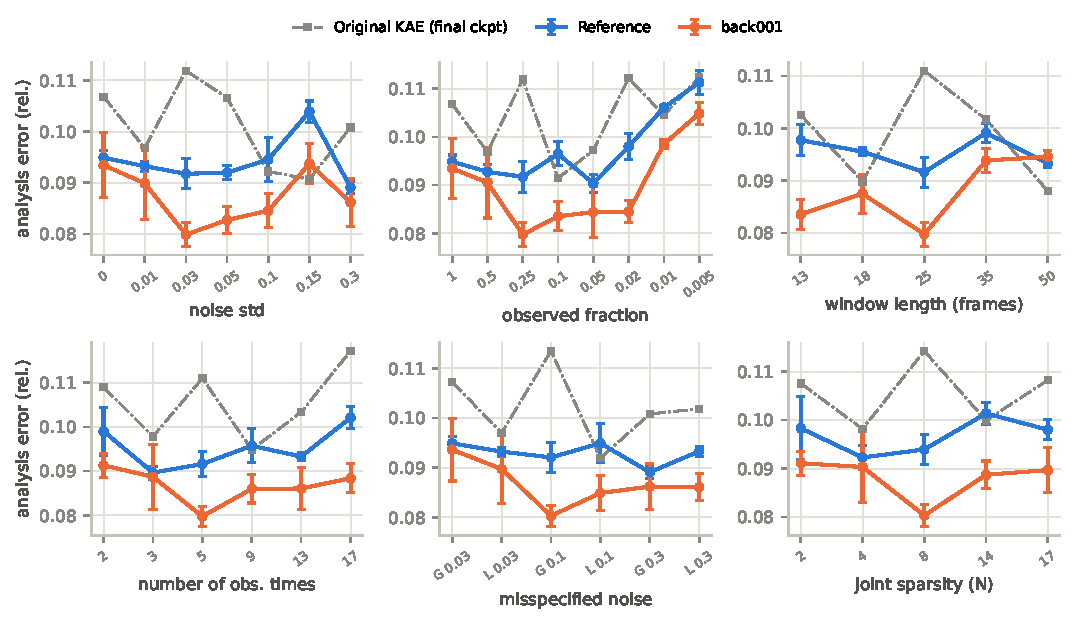
\includegraphics[width=\linewidth]{fig_cand_da.pdf}
\caption{DA analysis error over the six df9 sweeps, mean $\pm$ SE over 3 seeds; the original
KAE is its final checkpoint on the same DA code. ACDM and U-Net (0.26--0.27) are off scale.}
\label{fig:da}
\end{figure}

\begin{center}\small
\begin{tabular}{lcccccc}
\toprule
df9 sweep (3 seeds, paired) & points & reference & back001 & $\Delta\pm$SE & back001 better\\
\midrule
noise & 7 & 0.0942 & 0.0872 & $-0.0070\pm0.0044$ & 7/7\\
sparsity & 8 & 0.0977 & 0.0899 & $-0.0078\pm0.0035$ & 8/8\\
window length & 5 & 0.0955 & 0.0878 & $-0.0076\pm0.0027$ & 4/5\\
number of observation times & 6 & 0.0952 & 0.0867 & $-0.0085\pm0.0047$ & 6/6\\
misspecified noise & 6 & 0.0929 & 0.0868 & $-0.0061\pm0.0042$ & 6/6\\
joint sparsity & 5 & 0.0968 & 0.0880 & $-0.0088\pm0.0048$ & 5/5\\
\midrule
\textbf{all} & 37 & 0.0954 & \textbf{0.0878} & $\mathbf{-0.0076\pm0.0040}$ & \textbf{36/37}\\
\midrule
df1 headline (seed 0) & 1 & 0.0286 & 0.0254 & $-11\%$ & --\\
df1 sweeps (seed 0) & 47 & 0.041--0.047 & 0.030--0.035 & about $-25\%$ & 46/47\\
\bottomrule
\end{tabular}
\end{center}

\begin{itemize}
\item The gain is largest with noisy (0.1), heavy-tailed (Laplace) and sparse observations and
  short windows, and vanishes for the longest window (50 frames), where long-range forecast
  error dominates the misfit.
\item Seed caveat: seed 0 gains least ($-0.0001$ to $-0.003$); seeds 1--2 carry most of the
  improvement. df1 is seed 0 only, as for the reference.
\item \textbf{Not from observability.} The DA conditioning diagnostic shows unchanged observation
  gains (median 3.06 vs 2.98; 10th percentile 0.44 vs 0.44), a latent problem about 3$\times$
  \emph{worse} conditioned for the optimiser (condition number $6.7\times10^4$ vs
  $2.2\times10^4$), and a lower misfit at the analysis (0.0016 vs 0.0020, with the misfit of the
  true state 0.0024 for both: 4D-Var still prefers a wrong state). The gain comes from what the
  latent encodes, consistent with the lead-1 gain.
\end{itemize}

\subsection{Zero-shot time resolution and Mach sensitivity}
Trained on frames 0.1 apart, queried every 0.05 (3 seeds, MSE $\times10^{-3}$):
\begin{center}\small
\begin{tabular}{lcccc}
\toprule
 & int, half-step leads & int, whole-step leads & ext, half-step & ext, whole-step\\
\midrule
reference & 3.51 & 3.49 & 1.99 & 1.98\\
back001   & 3.16 & 3.15 & 2.11 & 2.10\\
$\Delta\pm$SE & $-0.35\pm0.14$ & $-0.35\pm0.14$ & $+0.12\pm0.25$ & $+0.12\pm0.25$\\
\bottomrule
\end{tabular}
\end{center}
Both models are as accurate at never-trained half steps as at trained steps. Output change
under a wrong Mach number (true 0.66) is nearly identical; back001 reacts slightly more at 0.90
(rms 0.76 vs 0.68).

%======================================================================
\section{The mixture readout}\label{sec:mix}

\begin{figure}[h]
\centering
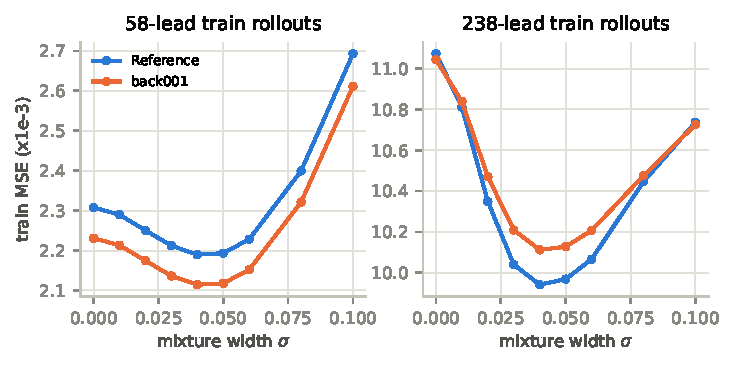
\includegraphics[width=0.75\linewidth]{fig_cand_sigma.pdf}
\caption{Calibration of the mixture width on training rollouts only (mean of 3 seeds).}
\label{fig:sigma}
\end{figure}

\begin{itemize}
\item \textbf{Why.} The wake is a noisy oscillator: its phase speed varies by about $\pm14\%$
  within a simulation and cannot be predicted from the input window ($R^2\approx0.19$ even from the
  full state). A single decode commits to one phase and is wrong at long leads.
\item \textbf{Calibration.} $\sigma\in\{0,\dots,0.10\}$ on 58-lead rollouts from two windows per
  training simulation; selected 0.04 / 0.04 / 0.05 for the reference seeds and the same for
  back001. No test data are used.
\item \textbf{Effect on the reference} (3 seeds, paired): ext $-0.14\pm0.04$, int $-0.22\pm0.03$,
  long $-3.04\pm0.31$; DA unchanged.
\item \textbf{Cost.} 5$\times$ the decoding at inference, and lower energy at long leads (about
  0.5--0.6 of the true fluctuation energy at lead 58), so LSiM gets worse: ext 1.41$\to$1.72,
  int 1.71$\to$1.87, long 4.06$\to$5.74 ($\times10^{-1}$).
\end{itemize}

%======================================================================
\section{Ablation study}\label{sec:abl}

Each variant changes one thing in the reference and is trained with the same seeds; entries are
the paired change against the reference run of the same seed (mean over seeds $\pm$ SE of the
paired change). Bold: improvement beyond 2 SE; $\dagger$: deterioration beyond 2 SE (2-seed
SEs are rough).

Tables~\ref{tab:abl1} and~\ref{tab:abl2} are on landscape pages at the end of this section.
DA learning rates were re-tuned wherever the optimum sat at the edge of the grid; every row's
optimum is now interior.

\begin{landscape}
\begin{table}[p]
\centering\scriptsize
\caption{Ablations, \textbf{single decode}. MSE $\times10^{-3}$ (all frames), LSiM $\times10^{-1}$,
DA = mean over the 26 points of the four df9 sweeps (window length, number of observation
times, sparsity, noise).}
\label{tab:abl1}
\resizebox{\linewidth}{!}{%
\begin{tabular}{lcccccccc}
\toprule
Variant & seeds & ext MSE & int MSE & long MSE & ext LSiM & int LSiM & long LSiM & DA df9\\
\midrule
\inputrows tab_abl_single.tex
\bottomrule
\end{tabular}}
\end{table}

\begin{table}[p]
\centering\scriptsize
\caption{Ablations, \textbf{mixture readout} (each checkpoint with its own train-calibrated
$\sigma$). DA is identical to Table~\ref{tab:abl1}. The dense and Hurwitz generators are absent:
the mixture rescales oscillator frequencies, which only the block generator has.}
\label{tab:abl2}
\resizebox{\linewidth}{!}{%
\begin{tabular}{lcccccccc}
\toprule
Variant & seeds & ext MSE & int MSE & long MSE & ext LSiM & int LSiM & long LSiM & DA df9\\
\midrule
\inputrows tab_abl_mix.tex
\bottomrule
\end{tabular}}
\end{table}
\end{landscape}

\textbf{What the ablations show} (single decode unless stated):
\begin{itemize}
\item \textbf{Mach conditioning is essential} (removing it: ext $+8.9$, int $+9.6$, DA
  $+0.096$). Conditioning only the generator (encoder and decoder Mach-free) is also worse
  (int $+0.31$, DA $+0.005$).
\item \textbf{The structured generator matters}: a dense unconstrained generator blows up long
  rollouts (long $+18$) and costs DA ($+0.024$); a Hurwitz generator costs DA ($+0.041$).
\item \textbf{Latent size 256 is right}: 128 is worse on int ($+0.45$) and DA ($+0.013$); 512
  is no better anywhere and worse on long with the mixture ($+2.27$).
\item \textbf{Two input frames matter}: one frame costs ext ($+0.77$) and int ($+0.25$).
\item \textbf{A Mach-dependent fixed point $\mu(\mathrm{Ma})$} helps int ($-0.31\pm0.11$; with the
  mixture $-0.26$) and leaves DA unchanged ($-0.001\pm0.001$), but costs ext and long slightly
  (with the mixture $+0.19$, $+0.36$). Not adopted; a candidate to combine with back001.
\item \textbf{Multi-step training and latent consistency are essential}; one-step training and
  removing the latent-consistency or prediction loss are worse on almost everything.
\item \textbf{Backward latent consistency is the only term that improves DA}, with a trade-off
  set by its weight: 0.1 gives DA $-0.018\pm0.003$ but ext $+1.14$, int $+0.77$; 0.01 (back001)
  keeps most of the DA gain at no cost on ext and a gain on int.
\item \textbf{Every regulariser and combination made DA worse}; the combinations (latent and Mach
  noise, with or without 4 of 8 leads) improve long ($-0.93$, $-1.37$) but cost DA
  ($+0.010$, $+0.009$).
\item \textbf{L1 instead of squared error is worse} (3 seeds): L1 for reconstruction and
  prediction DA $+0.027\pm0.006$, int $+2.00\pm0.55$; L1 for reconstruction only (the original
  KAE's setting) DA $+0.013\pm0.003$, int $+0.49\pm0.19$. L1 does not explain the original
  KAE's DA.
\item \textbf{Hedged readout} (a learned forecast decay separate from the state dynamics) was
  dropped before completion: the mixture readout supersedes it.
\end{itemize}

%======================================================================
\section{Post-processing study}\label{sec:pp}

\textbf{Goal:} the best possible forecasting numbers from the two candidates without changing
training or the linear latent model. Every technique is calibrated on training rollouts only
(238 leads from two windows per training simulation) and scored once on test.

\begin{center}\small
\begin{tabularx}{\linewidth}{lY}
\toprule
Technique & Idea\\
\midrule
Lead-dependent mixture width $\sigma(\tau)$ & phase uncertainty grows with lead; one width
  for all leads may be too narrow early or late\\
Wiener / MOS filter & per lead, channel and radial wavenumber, shrink the unpredictable part of
  the forecast anomaly towards an anchor; gain = regression of truth on forecast. Anchors: the
  forecast's own lead-1..58 mean (no extra data) and a Mach-interpolated training climatology\\
Scalar shrinkage & the same with one gain per lead and channel (checks whether scale dependence matters)\\
Seed ensembles & mean of the 3 seeds of a model, and of all 6 checkpoints; each member is still
  an exact linear model\\
Combinations & the above stacked\\
\bottomrule
\end{tabularx}
\end{center}

\textbf{Caveats.} The model fits training data much better than test data (\S\ref{sec:findings}),
so train-calibrated corrections are conservative. The training Mach numbers skip 0.64--0.68
(where int and long sit) and stop at 0.53 (ext is 0.50--0.52), so the climatology anchor must be
interpolated or extrapolated.

\subsection{Results}

Lab: 238-lead rollouts from two windows of each training simulation give the calibration
statistics for nine mixture widths; the test forecasts of all widths are stored once and
combined offline (\texttt{scripts/postproc/}). The plain mixture reproduces the stored test
scores exactly (reference seed 0: 1.534 / 3.124 / 13.214).

\begin{table}[h]
\centering\scriptsize
\caption{Post-processing variants, paired against the mixture readout of the same checkpoint (mean
over 3 seeds $\pm$ SE). First row: absolute all-frames MSE $\times10^{-3}$ of the mixture. Bold:
improvement beyond 2 SE; $\dagger$: deterioration beyond 2 SE. ``Own mean'': the forecast's mean
over leads 1--58; ``climatology'': Mach-interpolated time-mean of the training simulations.}
\label{tab:pp}
\begin{tabular}{lcccccc}
\toprule
 & \multicolumn{3}{c}{Reference} & \multicolumn{3}{c}{back001}\\
\cmidrule(lr){2-4}\cmidrule(lr){5-7}
Variant & ext & int & long & ext & int & long\\
\midrule
\inputrows tab_pp_delta.tex
\bottomrule
\end{tabular}
\end{table}

\begin{table}[h]
\centering\scriptsize
\caption{Seed ensembles: the field average of the 3 seeds of a model, or of all 6 checkpoints;
each member uses the variant named in the row. All-frames MSE $\times10^{-3}$.}
\label{tab:ppens}
\begin{tabular}{lccccccccc}
\toprule
 & \multicolumn{3}{c}{Reference, 3 seeds} & \multicolumn{3}{c}{back001, 3 seeds} &
   \multicolumn{3}{c}{All 6 checkpoints}\\
\cmidrule(lr){2-4}\cmidrule(lr){5-7}\cmidrule(lr){8-10}
Members & ext & int & long & ext & int & long & ext & int & long\\
\midrule
\inputrows tab_pp_ens.tex
\bottomrule
\end{tabular}
\end{table}

\begin{table}[h]
\centering\scriptsize
\caption{LSiM $\times10^{-1}$ (lower is better) for the shortlisted variants: mean over the 3
seeds, and of the 3-seed average.}
\label{tab:pplsim}
\begin{tabular}{llcccccc}
\toprule
 & & \multicolumn{2}{c}{ext} & \multicolumn{2}{c}{int} & \multicolumn{2}{c}{long}\\
\cmidrule(lr){3-4}\cmidrule(lr){5-6}\cmidrule(lr){7-8}
Model & Variant & seeds & average & seeds & average & seeds & average\\
\midrule
Reference & mixture            & 1.72 & 1.75 & 1.87 & 1.86 & 5.74 & 6.07\\
          & + shrink to clim.  & 1.78 & 1.81 & 1.91 & 1.91 & 7.00 & 7.10\\
          & + Wiener to clim.  & 1.80 & 1.82 & 1.91 & 1.91 & 6.85 & 6.97\\
\midrule
back001   & mixture            & 1.81 & 1.85 & 1.83 & 1.82 & 6.09 & 6.50\\
          & + shrink to clim.  & 1.86 & 1.90 & 1.87 & 1.85 & 7.23 & 7.35\\
          & + Wiener to clim.  & 1.89 & 1.93 & 1.86 & 1.85 & 7.04 & 7.20\\
\midrule
\multicolumn{2}{l}{\emph{Single decode, one seed (for reference)}} & 1.41 & -- & 1.71 & -- & 4.06 & --\\
\multicolumn{2}{l}{\emph{ACDM / U-Net$_{ut}$}} & 1.29 / 1.09 & & 1.38 / 0.95 & & 3.83 / 3.81 & \\
\bottomrule
\end{tabular}
\end{table}

\FloatBarrier
\textbf{What works.}
\begin{itemize}
\item \textbf{Seed averaging is the largest gain.} The 3-seed average of the mixture forecasts
  lowers ext by 0.19 (both models), int by 0.22--0.23 and long by 0.36 (reference) and 0.50
  (back001) against the single-seed mean. The reference's 3-seed average (1.58) is ahead of
  U-Net$_{ut}$ on ext (1.60); back001's (2.67) is ahead of ACDM on int (2.92). Averaging all six
  checkpoints is no better than the better 3-seed average on any case.
\item \textbf{Climatology shrinkage helps long only}: $-0.90\pm0.05$ (reference) and
  $-1.23\pm0.05$ (back001), paired; on the 3-seed averages $-0.70$ and $-0.91$. The calibrated
  gains stay close to 1 up to lead 58, so ext and int barely move ($\le0.03$). It helps back001
  more, which nearly closes back001's long deficit (12.22 vs 12.13, single-seed means).
\item \textbf{Scale dependence adds nothing}: the per-wavenumber Wiener filter and one scalar per
  lead and channel are within 0.03 of each other; the scalar is the simpler choice.
\end{itemize}

\textbf{What does not.}
\begin{itemize}
\item \textbf{A lead-dependent mixture width} is no better (reference long $+0.11\pm0.03$): the
  train-optimal width is 0.02 for the first leads and close to the calibrated one after lead 30,
  and the first leads carry little error.
\item \textbf{Shrinking towards the forecast's own mean} gives 30--60\% of the climatology gain
  ($-0.26$ to $-0.72$ on long). Applied to the single decode instead of the mixture, it is worse
  on ext and int ($+0.02$ to $+0.03$ against the mixture) and only matches it on long for the
  reference.
\end{itemize}

\textbf{Costs.} All of it lowers LSiM quality: shrinkage adds 0.95--1.26 ($\times10^{-1}$) on
long and 0.03--0.08 on ext and int, and seed averaging adds a little more on ext and long, because both reduce the
fluctuation energy of uncertain forecasts. Seed averaging triples inference. Neither changes the
data assimilation, which uses the latent model of one checkpoint; DA with a seed ensemble (three
independent 4D-Var analyses, averaged) has not been run.

\callout{\textbf{Post-processing to report.} Primary: 3-seed average + mixture + scalar
climatology shrinkage, calibrated on training rollouts. Report single-model numbers and LSiM
alongside it.}

%======================================================================
\section{Findings from the investigation}\label{sec:findings}
\begin{itemize}
\item \textbf{The wake is a noisy oscillator.} Phase speed varies by about $\pm14\%$ within a
  simulation and is unpredictable from the window ($R^2\approx0.19$); $\omega(\mathrm{Ma})$ is
  jagged; about 29 oscillator pairs within $\pm20\%$ of the shedding frequency carry 66\% of the
  latent variance.
\item \textbf{Long-lead hedging is dephasing, not damping}, and averaging decodes in pixel space,
  $\mathbb E[D(z)]$, beats shrinking the latent, $D(\mathbb E[z])$. This is the basis of the
  mixture readout.
\item \textbf{The short-lead floor is a generalisation gap}, not a capacity limit: reconstruction
  error 0.004--0.07 on training simulations against about 0.35 on Tra\_int; a 256-mode POD
  reaches 0.20.
\item \textbf{DA error is identifiability and overfitting of model error.} An oracle test shows
  the model's trajectory family can fit both $t_0$ and the future; plain 4D-Var instead fits the
  observations with a wrong $t_0$. Removing damping at DA time (0.0958 vs 0.0963) or warping the
  phase speed (0.0961 / 0.0957) does not help. The backward term (tested at weight 0.1) cuts the
  oracle future misfit from 0.040 to 0.015, the likely mechanism behind back001's DA gain.
\end{itemize}

%======================================================================
\section{Open items}
\begin{itemize}
\item DA with a seed ensemble (average of three 4D-Var analyses), to see whether the ensemble
  gain carries over to DA.
\item back001 combined with the conditional fixed point $\mu(\mathrm{Ma})$ (both help int; neither
  hurts DA).
\item Next candidates, not yet run: a POD-backbone decoder (attacks the generalisation gap);
  leave-block-out Mach conditioning; training with the mixture readout inside the loss;
  test-time refinement of $z_0$ on the input frames; a tied quadrature multiplet.
\item Paper: switch the main tables to the chosen CT-KAE and its DA results (\texttt{da\_v3}).
\end{itemize}

\end{document}
